\chapter{Theory}
% Indholds fortegnelse til teori: 
% \begin{itemize}
% \item NF teori
% %\rod{   \subitem porøsitet + construction af hollow fiber membran + flow}
%         \subitem TMP + flux formler 
%         \subitem Concentration polarisering 
%         \subitem rejection
%         \subitem osmotisk tryk
%         \subitem fouling scaling 

% \item Ioner, samspil og hvad påvirker dem
%     \subitem 3 faktore: ligevægt, sterisk hindring og ladning (negative rejection). 
% \rod{\subitem pH-pC diagrammer. 
%     \subitem Chlorid
%     \subitem Silica 
% \item carbonat system 
%     \subitem buffer teori
%     \subitem titrering? 
%     %\subitem batch vs. continous.  
% \item "The Model" 
%     \subitem process regulering (formler) 
%     \subitem måske noget numerisk løsning (euler)
%     \subitem masse balancer mm. 
% }
% \end{itemize}





\section{Pressure driven filtration}
Filtration  is based on the retention of solutes and permeation of water.
%Rejection of trace ionic solutes in nanofiltration: Influence of aqueous phase composition:
NF membranes typically have a composite structure consisting of a thin active porous top-layer supported by a low resistance layer and are often used for removal of ions, taking advantage of the different ion membrane selectivities and greater water permeation than in RO.
This permeation of water though a semipermeable membrane can be described by the flux of water, \textit{J}, based on membrane resistance \textit{$R_m$} and is typically based on the permeate flow $Q_p$ per membrane area $A$ during operation:
\begin{ceqn}
    \begin{align}
        J=\frac{\Delta P}{\mu R_m}=\frac{Q_p}{A}
    \end{align}
\end{ceqn}



Where $\Delta P $ is the pressure drop through the membrane which is the primary driving force of the water permeation. %max klunt
This trans-membrane pressure is defined as the average pressure on the inlet side (feed and retentate streams) minus the pressure on the permeate stream. 
\begin{ceqn}
    \begin{align}
        \Delta P=\frac{P_{feed}+P_{retentate}}{2}-P_{permeate}
    \end{align}
\end{ceqn}



As NF uses semipermeable membranes which separates a stream with solutes and a purer stream there is a difference in chemical potential between the two streams which is also known as the osmotic pressure $\pi$ described by \cref{eq:osmotic_pressure}:
\begin{ceqn}
    \begin{align}
    \label{eq:osmotic_pressure}
       \pi = \sum_{i=1} a_ic_iRT 
    \end{align}
\end{ceqn}
Here \textit{c} is the concentration of species $i$ in $mol/L$ , $a_i$ is the van't hoff factor which describes colligative properties of the dissolved specie. 
For ions and other electrolytes the dissociation is total and \textit{a} is effectively 1.
\textit{R} is the gas constant and \textit{T} is temperature in Kelvin. 
In NF the osmotic pressure has a great impact on performance and cannot be neglected.
Accounting for osmotic pressure the flux is given by:
\begin{ceqn}
    \begin{align} 
        J=\frac{(\Delta P-\Delta \pi)}{\mu R_m}
        \label{eqn:flux_including_osmotic_pressure}
    \end{align}
\end{ceqn}

Increasing pressure difference the flux will increase but also the concentration at the membrane wall causing an increase in osmotic pressure. 
For the retentate to be in equilibrium with the permeate stream there must be an applied pressure equal to this osmotic pressure.
Therefore the driving force required changes depending on the quality of the feed stream as the force has to overcome the difference in osmotic pressure plus the pressure necessary to transport the water.
The osmotic pressure experienced by the membrane is not due to bulk concentration but rather the concentration at the membrane wall which is higher due to the rejection of the solutes.
% This means that the applied pressure is higher than the net applied pressure (NAP): $NAP=\Delta P-\Delta \pi=P_{net}$
 



% Solute flux based on mass transfer coeff:
% \begin{ceqn}
%     \begin{align}
%     F_s=K_s(c_m-c_p)=K_s[(\frac{c_f+c_c}{2})-c_p]=\frac{Q_pc_p}{A}
%     \end{align} 
%  \end{ceqn}


\subsection{Solute Retention }
The primary purpose of a membrane is to retain solutes. 
The degree to which a membrane accomplished this can be expressed by the membrane rejection, Rej, of a given species described as the ratio between the feed and permeate concentrations of the solute. \cref{eq:rejection_formula}.
\begin{ceqn}
    \begin{align}
    \label{eq:rejection_formula}
       Rej = 1 - \frac{c_p}{c_f} 
    \end{align}
\end{ceqn}
$c_p$ describes the concentration of a species in the permeate stream and $c_f$ describes the concentration in the feed stream. 
The rejection of different species/ions for a given membrane sometimes varies quite dramatically and is influenced by a variety of factors.
%Detailed descriptions in the mechanisms behind solute rejection in NF are presented in \Cref{ion_afsnit}.  
Typically the intrinsic rejection ($R_int$)is higher than the observed rejection which is determined in relation to the bulk concentration.  
This is due to the partial rejection of solutes by membranes, whereby accumulation occurs near the membrane walls and solutes are present at an increased concentration compared to the bulk ($c_m > c_f$).
This is known as concentration polarisation (CP) and results in a boundary layer of increased concentration at the membrane wall see \cref{fig:flux_concentration_polerization_cp}.

Near the membrane wall a laminar boundary layer exist where mass transport is governed by film theory.
Solutes are brought to the membrane by convection and removed by a diffusive flow away from the membrane
\citep{mulderBasicPrinciplesMembrane1996}
see figure \cref{fig:flux_concentration_polerization_cp}.
The severity of CP is inversely dependent on the mass transfer coefficient ( $k=D/\delta$) as the concentration at the membrane wall increases at low mass transfer coefficients.
\Cref{eqn:CP_mass_transfer_modulus} is the CP modulus and describes the ratio between concentration at the membrane wall and in feed bulk solution.
 \begin{ceqn}
    \begin{align}
     \frac{c_m}{c_f}=\frac{\exp{(J/k)}}{R_{int}+(1-R_{int})\exp{(J/k)}} 
     \label{eqn:CP_mass_transfer_modulus}
     \end{align}
 \end{ceqn}
From this equation it is apparent that mainly flux and mass transfer are responsible for CP.
Therefore both membrane properties and hydrodynamics affect the severity of CP.
CP can therefore be reduced by increasing cross flow over the membrane to change the mass transfer coefficient through the boundary layer. \citep{seaderSeparationProcessPrinciples2006}

 
 \begin{figure}[H]
     \centering
    \begin{tikzpicture}[scale=0.7]
\coordinate (A) at (8,0);
\coordinate (B) at (5,2);
\coordinate (C) at (8,5);
\draw  (0,0) node[below]{$x$} --(A) node[below]{0};
\draw (0,2) node[above]{$c_f$} -- (B);
\draw[dashed] (B)--+(0,5)--+(0,-2) node[below]{$\delta$};
\draw[pattern=north east lines, pattern color=blue] (A) rectangle +(0.8,6);
\draw (B) to[out=0,in=270] (C) node[left]{$c_m$};
\draw (8.8,0.5)--node[above]{$c_p$}++(2,0);
\draw[   decoration={markings,
        mark=at position 1 with {\arrow[scale=2.5,>=latex]{>}}
        },
    postaction={decorate}] (5.5,4)--node[above]{$J\cdot c$}++(1.5,0);
\draw[   decoration={markings,
        mark=at position 1 with {\arrow[scale=2.5,>=latex]{>}}
        },
    postaction={decorate}] (7.5,1)--node[above]{$D\cdot \frac{dc}{dx}$}++(-1.5,0);

\draw[   decoration={markings,
        mark=at position 1 with {\arrow[scale=2.5,>=latex]{>}}
        },
    postaction={decorate}] (9.5,4)--node[above]{$J\cdot c_p$}++(1.5,0);

\node at (2,6) {Bulk Feed};
\node at (6.6,6.2) {Boundary};
\node at (6.6,5.8) {Layer};
\end{tikzpicture}
     \caption{Concentration and CP. With inspiration from \citep{mulderBasicPrinciplesMembrane1996}}
     \label{fig:flux_concentration_polerization_cp}
 \end{figure}
 
 
CP can affect selectivity and performance of membranes quite significantly. \citep{deonConcentrationPolarizationPhenomenon2013}
The increased concentrations influence the performance by increasing the osmotic pressure and thereby the required driving force according to \Cref{eq:osmotic_pressure,eqn:flux_including_osmotic_pressure} or reducing flux.
Osmotic pressure along with CP is responsible for the limiting flux behaviour seen when increasing applied pressure.
% In such cases scaling or precipitation of gel layers may form on the membrane reducing the flux through the membrane \citep{seaderSeparationProcessPrinciples2006}
% (see \Cref{Fouling} for more on fouling).
CP is especially critical for membrane performance when the retained solutes reach concentrations close to their solubility limits near the membrane wall.
Therefore CP is often a precursor to fouling.
  
\subsection{Fouling}
\label{Fouling}
Membrane fouling is the deposition of suspended or dissolved solute on the membrane surface resulting in reduced performance.
Fouling can substantially decrease permeability, increase operational cost and shorten membrane life, and is the biggest obstacle in membrane filtration processes. 
\citep{nanofiltration_2021_bog_fraMorten} 
Passing feed directly to the NF/RO membrane might cause irreversible fouling, which is why pretreatment is often implemented \citep{farahanniRecoveryCoolingTower_2016}.
Some part of fouling is reversible and performance may be regained by simple hydraulic cleaning  while another part of fouling is irreversible and can only be remedied by chemical cleaning or not at all \citep{seaderSeparationProcessPrinciples2006,nanofiltration_2021_bog_fraMorten}.
Typically scaling is the major cause for irreverisble fouling.%er måske for meget uden en kilde

Scaling is a special case of fouling caused by solutes exceeding their solubility limits and precipitating on the membrane surface.
Other fouling origins include deposition of colloidal solutes, chemical reaction leading to precipitation, gel formation, biofouling, etc. 
In real life conditions multiple mechanisms are at play at the same time although most research is focused on one mechanism at a time \citep{nanofiltration_2021_bog_fraMorten}.
Calcium carbonate, gypsum, barium/strontium sulphate and silica are the most common constituents of scale on NF membranes \citep{vanderbruggenDrawbacksApplyingNanofiltration2008}.


One way to asses the degree of membrane fouling is by finding the flux reduction (FR) of a membrane.
This is done by comparing the pure water flux of the unfouled membrane($J_{v,a}$) with its performance after operation at the same pressure ($J_{v,b}$):  
\begin{ceqn}
    \begin{align}
        FR = \frac{J_{v,b}-J_{v,a}}{J_{v,b}}*100 (\%)
    \end{align}
\end{ceqn}
When FR reaches some critical value the membrane will be considered fouled and it will have to be cleaned, often by chemical cleaning. 
This should be done according to the manufacturer recommendation, e.g. NX Filtration recommends cleaning after observing FR of 30\%. \citep{NXfiltration_operation_manual} 
Chemical cleaning typically consists of exposing the membrane to alkaline and acidic solutions in order to dissolve and remove foulants.
If the solution is circulated over the membrane it is a chemically enhanced flush (CEF) if the membrane is soaking in the membrane it is a cleaning in place (CIP) procedure.  \citep{NXfiltration_operation_manual}

% \begin{figure}[H]
%     \centering
%     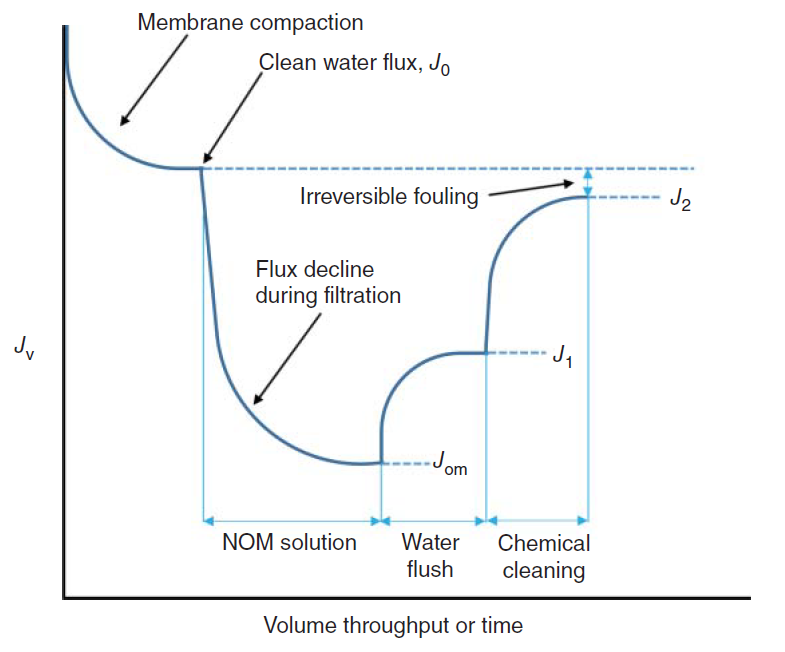
\includegraphics[width=0.7\textwidth]{Billeder/teori/fouling_flux.png}
%     \caption{Typical flux (constant pressure) \citep{nanofiltration_2021_bog_fraMorten}}
%     \label{fig:flux_fouling}
% \end{figure}